%
%
%
%
%

\StartChapter[ch:anhang]{Anhang}
\tcbset{breakable}
\renewcommand{\BreakIfNotEnoughSpace}{}
\renewcommand{\BreakIfNotEnoughSpaceChapter}{}
\SubsectionBar{Reib- und Formschluss}
\ZSFindex{Reibschluss}
\ZSFindex{Formschluss}

\ZSFReibschlussFormschlussTabelle

\SubsectionBar[sec:wnv-uebersicht]{WNV-Übersicht (Bauformen erkennen)}
\ZSFindex{Welle-Nabe-Verbindung!Bauformen}

% --- Formschluss: Übersichtsgrid + Vergleichspaar (Mitnehmer) ---
\begin{tablebox}[Formschlüssige WNV\ZSFTitleTag{\ZSFref{sec:wnv-formschluss}}]
  \setlength{\tabcolsep}{2pt}%
  \begin{ZSFtablePlain}{Z{0.78} Y{1.22} Z{0.78} Y{1.22}}
    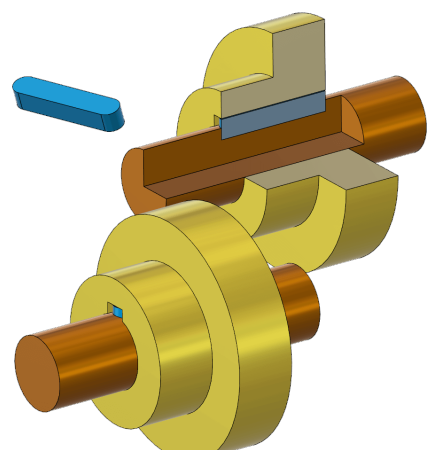
\includegraphics[width=13mm,keepaspectratio]{graphics/wnv_passfeder.png} &
    {\ZSFReadableOn \ZSFkeyword*{Passfeder}\newline 1 Mitnehmer $\Rightarrow$ kleine Momente, günstig} &
    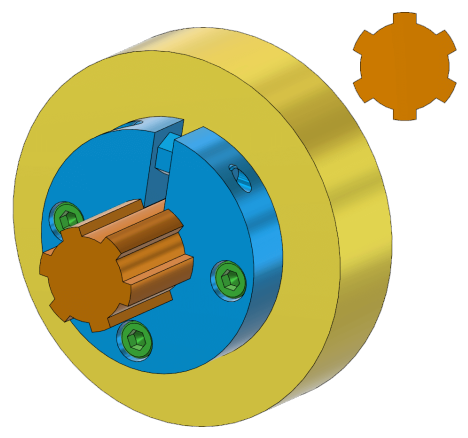
\includegraphics[width=13mm,keepaspectratio]{graphics/wnv_keilwelle.png} &
    {\ZSFReadableOn \ZSFkeyword*{Keilwelle}\newline mehrere Mitnehmer $\Rightarrow$ hohe Momente, teuer} \\
  \end{ZSFtablePlain}
  \ZSFgapXS
  {\centering
  \begin{tikzpicture}
    \node[anchor=south west,inner sep=0] (im) at (0,0)
      {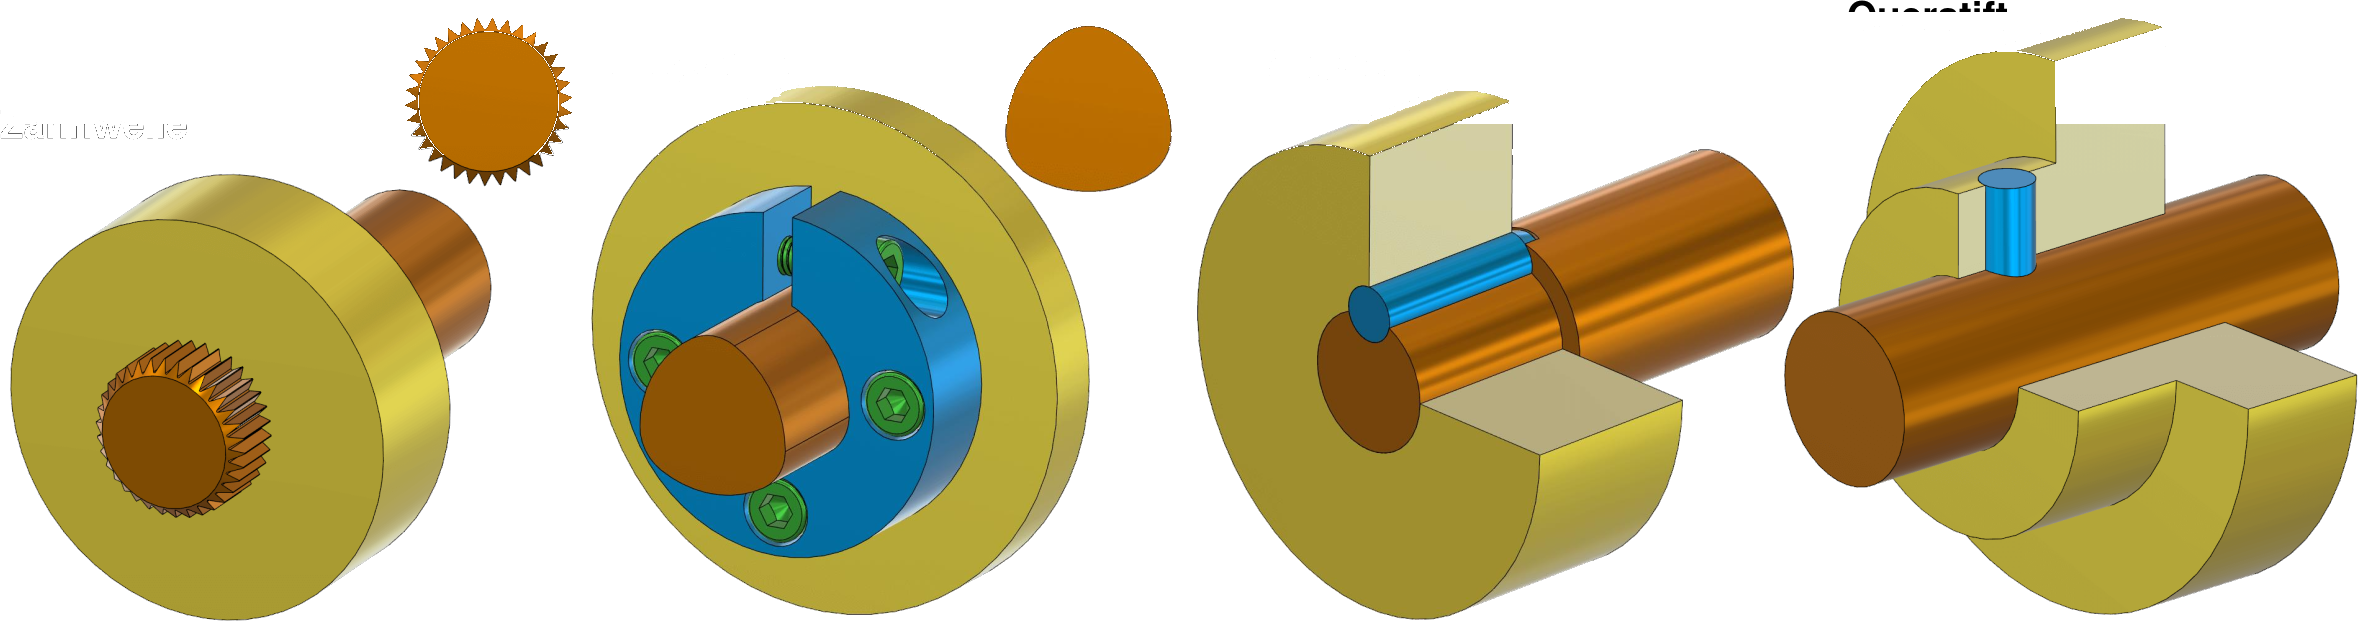
\includegraphics[width=0.72\linewidth,keepaspectratio]{graphics/wnv_uebersicht_formschluss.png}};
    \begin{scope}[x={(im.south east)},y={(im.north west)},
      every node/.style={font=\sffamily\bfseries\fontsize{5}{5.5}\selectfont,
        inner sep=0.5pt, fill=white, fill opacity=0.82, text opacity=1, rounded corners=0.5pt}]
      \node at (0.12,0.87) {Zahnwelle};
      \node at (0.37,0.66) {Polygonprofil};
      \node at (0.62,0.87) {Längsstift};
      \node at (0.88,0.66) {Querstift};
    \end{scope}
  \end{tikzpicture}\par}%
\end{tablebox}
\ZSFindex{Passfeder}
\ZSFindex{Keilwelle}
\ZSFindex{Zahnwelle}
\ZSFindex{Polygonprofil}
\ZSFindex[langsstift]{Längsstift}
\ZSFindex{Querstift}

% --- Reibschluss: Vergleichspaar (Pressverbände) + Übersichtsgrid ---
\begin{tablebox}[Reibschlüssige WNV\ZSFTitleTag{\ZSFref{sec:wnv-reibschluss}}]
  \setlength{\tabcolsep}{2pt}%
  \begin{ZSFtablePlain}{Z{0.78} Y{1.22} Z{0.78} Y{1.22}}
    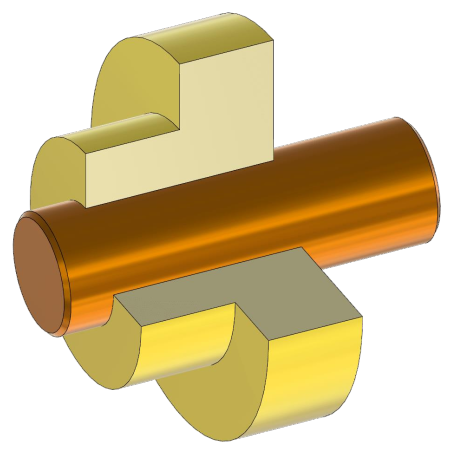
\includegraphics[width=13mm,keepaspectratio]{graphics/wnv_zpv.png} &
    {\ZSFReadableOn \ZSFkeyword*{Zylindr.\ Pressverband} \ZSFref{sec:zpv}\newline Übermass $\Rightarrow$ nicht lösbar, günstig} &
    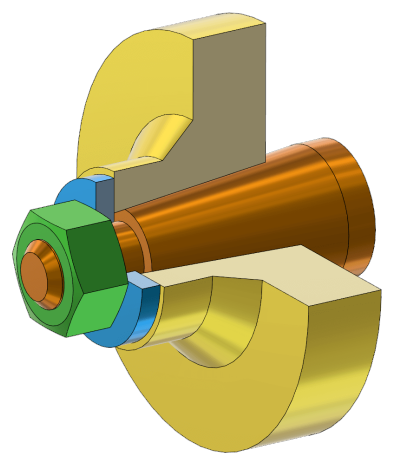
\includegraphics[width=13mm,keepaspectratio]{graphics/wnv_kpv.png} &
    {\ZSFReadableOn \ZSFkeyword*{Kegelpressverband} \ZSFref{sec:kpv}\newline Schraube $\Rightarrow$ lösbar/nachstellbar, teuer} \\
  \end{ZSFtablePlain}
  \ZSFgapXS
  {\centering
  \begin{tikzpicture}
    \node[anchor=south west,inner sep=0] (im) at (0,0)
      {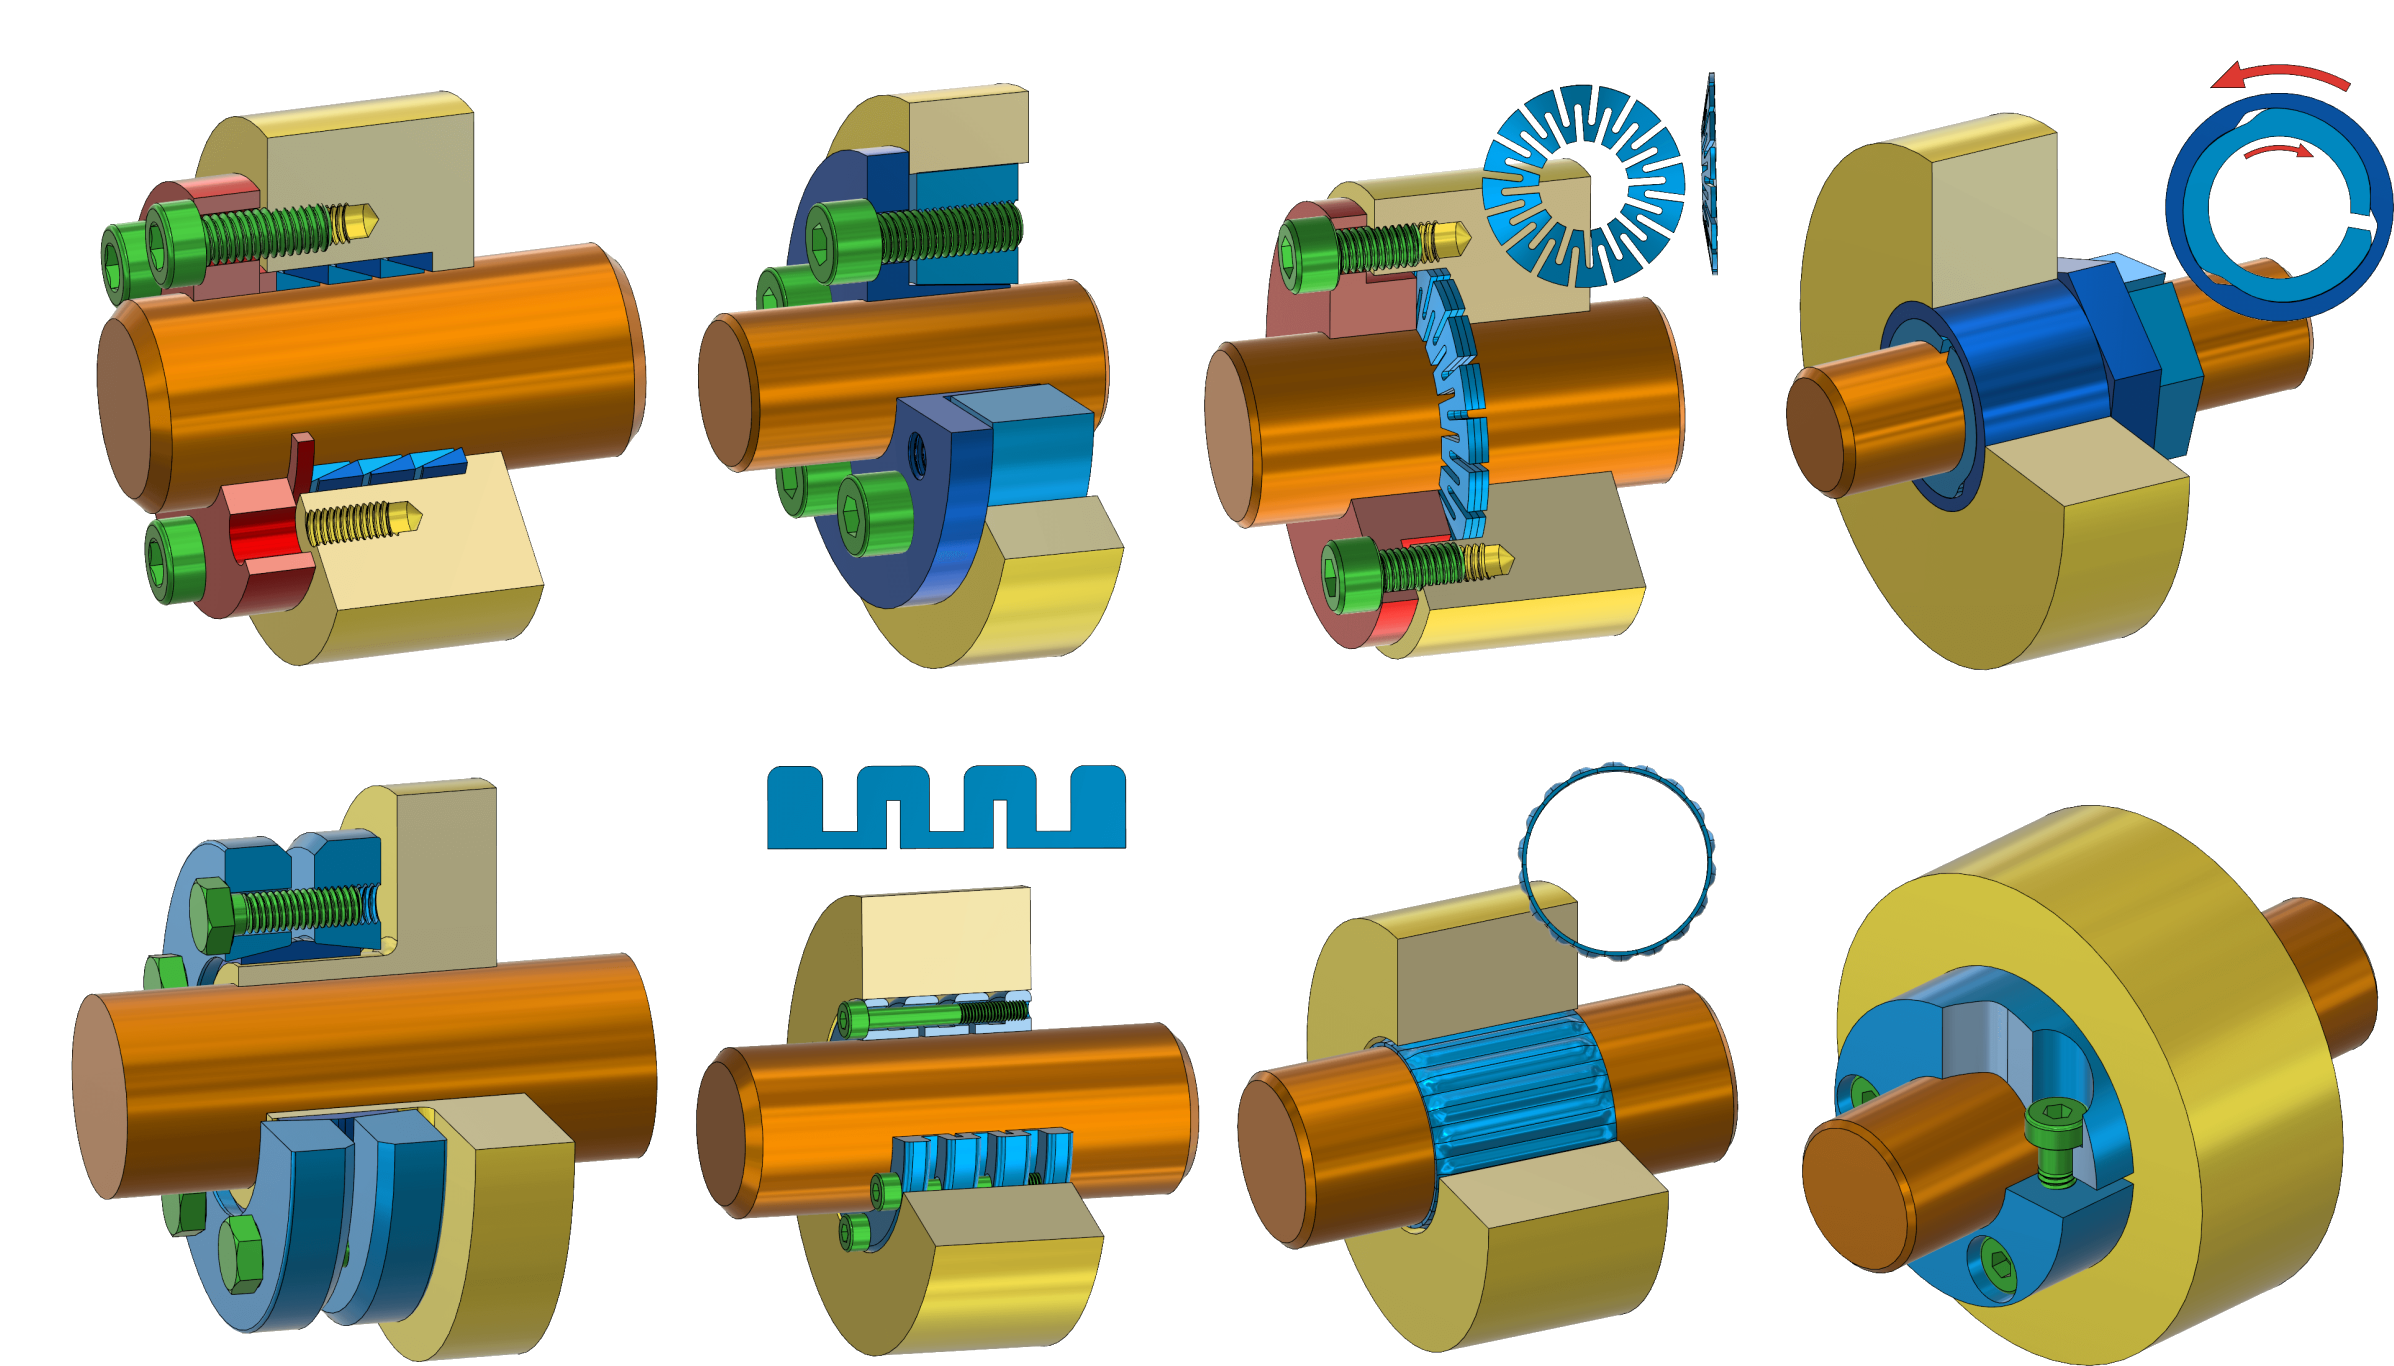
\includegraphics[width=0.72\linewidth,keepaspectratio]{graphics/wnv_uebersicht_reibschluss.png}};
    \begin{scope}[x={(im.south east)},y={(im.north west)},
      every node/.style={font=\sffamily\bfseries\fontsize{5}{5.5}\selectfont,
        inner sep=0.5pt, fill=white, fill opacity=0.82, text opacity=1, rounded corners=0.5pt}]
      \node at (0.13,0.965) {Kegelspannelemente};
      \node at (0.37,0.885) {Kegelspannsatz};
      \node at (0.62,0.965) {Sternscheiben};
      \node at (0.87,0.885) {Kreiskeilverbindung};
      \node at (0.13,0.505) {Schrumpfscheibe};
      \node at (0.37,0.425) {Druckhülse};
      \node at (0.62,0.505) {Toleranzring};
      \node at (0.87,0.425) {Klemmverbindung};
    \end{scope}
  \end{tikzpicture}\par}%
\end{tablebox}
\ZSFindex{Kegelspannelemente}
\ZSFindex{Kegelspannsatz}
\ZSFindex{Sternscheiben}
\ZSFindex{Kreiskeilverbindung}
\ZSFindex{Schrumpfscheibe}
\ZSFindex[druckhulse]{Druckhülse}
\ZSFindex{Toleranzring}
\ZSFindex{Klemmverbindung}

\SubsectionBar[sec:anziehwert]{Anziehwert $\ZSFscrewKA$}
\ZSFindex{Anziehwert}

\ZSFfig[1.0]{graphics/schrauben_anziehwert_ka_tabelle.png}{}{}

\SubsectionBar[sec:nachgiebigkeiten-orte]{Orte der einzelnen Nachgiebigkeiten}

\ZSFfig[0.47]{graphics/schraubenverbindung_nachgiebigkeit_bauteile.png}{}{}

\columnbreak

\SubsectionBar{Lager-Eignungsvergleich}
\ZSFindex{Wälzlagerwahl}
\ZSFindex{Lagereignung}

\ZSFfig[1.0]{graphics/lager_eignung.pdf}{}{}

\SubsectionBar[sec:momverlaeufe]{Dimensionierung \& Momentenverläufe}
\ZSFindex{Momentenverlauf}
\ZSFindex{Welle!Dimensionierung}

\begin{tablebox}[Standard-Lastfälle \& Vorgehen]
  \ZSFReadableOn
  \textbf{Regel}:~Nicht die ganze Welle berechnen -- nur kritische Stellen: kleine $\ZSFstressD$, hohe $\ZSFstressMb$, grosse Kerbwirkungen.\par
  \textbf{Superposition}:~Mehrere Momentenverläufe $\Rightarrow$ $\ZSFstressSigmaV$ an der Stelle max. Auslastung auswerten (kleinstes $\ZSFstressD$, höchstes $\ZSFstressMb$, schärfste Kerbe).
  \par\vskip\ZSFspaceXS
  \setlength{\tabcolsep}{1.0pt}%
  \begin{ZSFtablePlain}{Z{1.0} Z{1.0} Z{1.0}}
    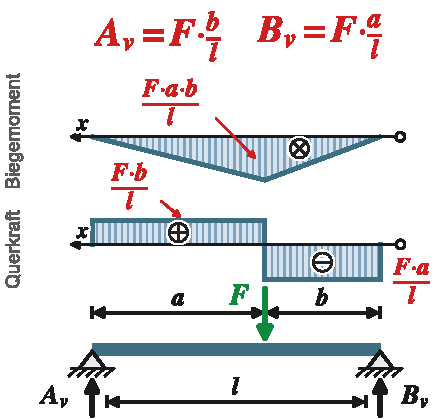
\includegraphics[width=0.98\linewidth]{graphics/momv_1.pdf} &
    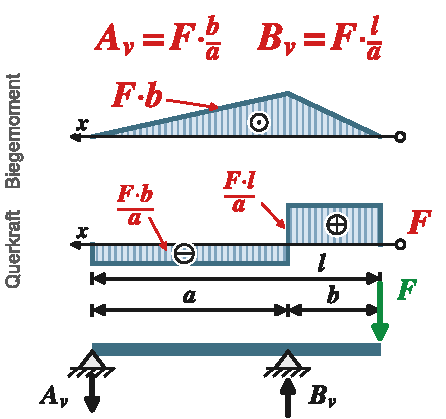
\includegraphics[width=0.98\linewidth]{graphics/momv_2.pdf} &
    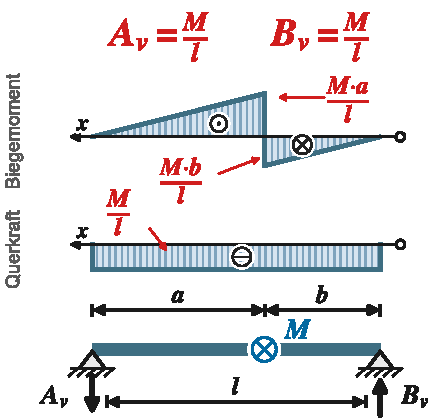
\includegraphics[width=0.98\linewidth]{graphics/momv_3.pdf} \\
    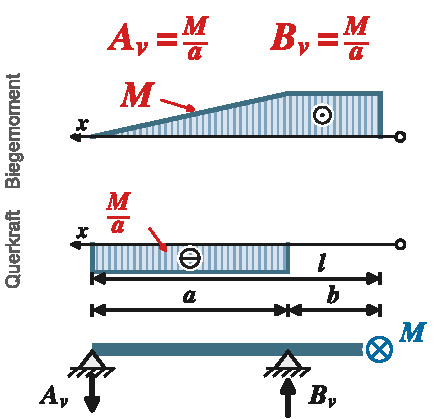
\includegraphics[width=0.98\linewidth]{graphics/momv_4.pdf} &
    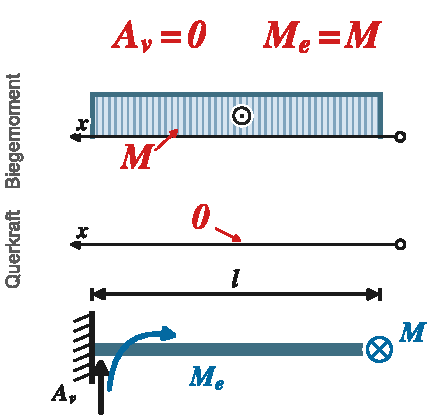
\includegraphics[width=0.98\linewidth]{graphics/momv_5.pdf} &
    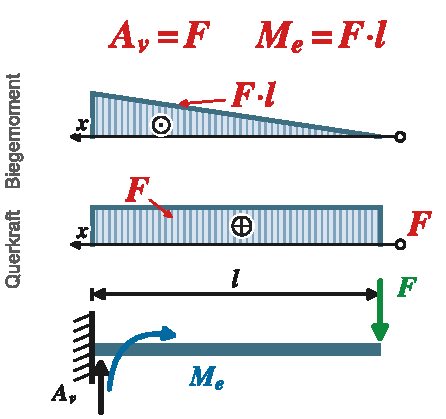
\includegraphics[width=0.98\linewidth]{graphics/momv_6.pdf} \\
    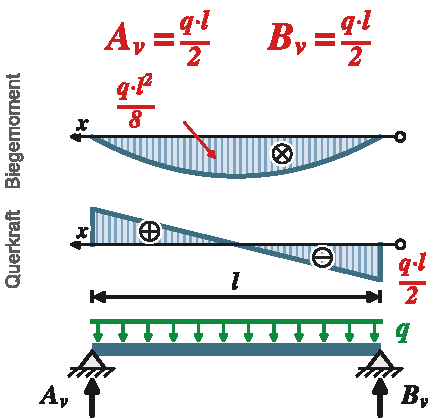
\includegraphics[width=0.98\linewidth]{graphics/momv_7.pdf} &
    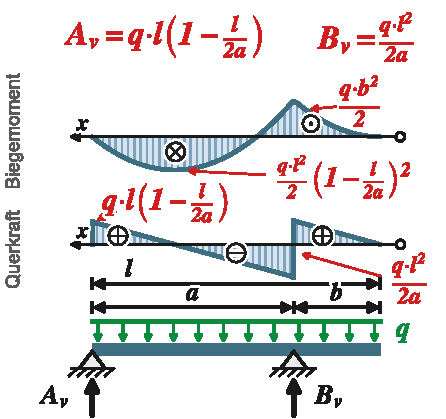
\includegraphics[width=0.98\linewidth]{graphics/momv_8.pdf} &
    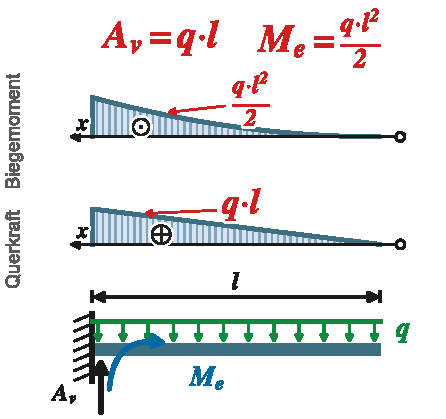
\includegraphics[width=0.98\linewidth]{graphics/momv_9.pdf}
  \end{ZSFtablePlain}
\end{tablebox}

\SubsectionBar[sec:cam-typ]{Kurvenscheiben-Typ (Cam) bestimmen}
\ZSFindex{Kurvenscheibe}
\ZSFindex{Cam}

\begin{defbox}[Kurvenscheiben-Typ (Cam) bestimmen]
  \ZSFReadableOn
  \ZSFkeyword*{Code}:~\textcolor{MechRoleBlue}{\textbf{D}} = \ZSFkeyword{Dwell} (Radius konst. $\Rightarrow$ Stössel ruht), \textcolor{MechRoleGreen}{\textbf{R}} = \ZSFkeyword{Rise} (Radius $\uparrow$), \textcolor{MechRoleRed}{\textbf{F}} = \ZSFkeyword{Fall} (Radius $\downarrow$). $\text{Drehzahl } n = \text{konst.} \Rightarrow$ nur Kontur zählt.
  \par\vskip\ZSFspaceXS
  \setlength{\tabcolsep}{1.0pt}%
  \begin{ZSFtablePlain}{Z{1.0} Z{1.0} Z{1.0} Z{1.0}}
    
\includegraphics[width=0.55\linewidth,keepaspectratio]{graphics/cam_d.pdf} &
    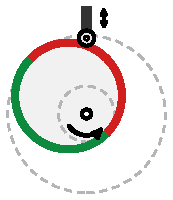
\includegraphics[width=0.55\linewidth,keepaspectratio]{graphics/cam_rf.pdf} &
    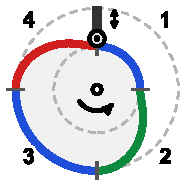
\includegraphics[width=0.55\linewidth,keepaspectratio]{graphics/cam_drdf.pdf} &
    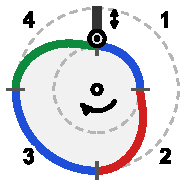
\includegraphics[width=0.55\linewidth,keepaspectratio]{graphics/cam_rdfd.pdf} \\
    {\ZSFfontNote \textcolor{MechRoleBlue}{\textbf{D}}: Kreis konz. $\Rightarrow$ Stössel ruht} &
    {\ZSFfontNote \textcolor{MechRoleGreen}{\textbf{R}}--\textcolor{MechRoleRed}{\textbf{F}}: Exzenter, kein Dwell} &
    {\ZSFfontNote \textcolor{MechRoleBlue}{\textbf{D}}--\textcolor{MechRoleGreen}{\textbf{R}}--\textcolor{MechRoleBlue}{\textbf{D}}--\textcolor{MechRoleRed}{\textbf{F}}: Ziff. = Ber.} &
    {\ZSFfontNote \textcolor{MechRoleGreen}{\textbf{R}}--\textcolor{MechRoleBlue}{\textbf{D}}--\textcolor{MechRoleRed}{\textbf{F}}--\textcolor{MechRoleBlue}{\textbf{D}}: andersrum $\Rightarrow$ inv. + \textcolor{MechRoleGreen}{\textbf{R}} $\leftrightarrow$ \textcolor{MechRoleRed}{\textbf{F}}}
  \end{ZSFtablePlain}
\end{defbox}

\ZSFStartClosingSubsection
\SubsectionBar*{Schlusswort}

\begin{statementbox}
Ich wünsche allen viel Erfolg bei der Prüfung!\par\ZSFgapXS

Den fachlichen Grundstein zu dieser ZSF haben meine Kollegen \ZSFkeyword{Liv Erne} und \ZSFkeyword{Silvio Seiz} gelegt. Ohne die beiden gäbe es diese Zusammenfassung nicht. Ich habe mein eigenes \ZSFkeyword{Hliddal Template} verwendet und hier und da noch ein paar kleine Dinge nach meinem Ermessen angepasst.

\ZSFgapS
\noindent\textbf{Links \& Ressourcen:}
\\
\textbf{Aktuelle Version \& Hliddal Template:}\\
\href{https://garcon-studios.ch/zsf}{garcon-studios.ch/zsf}
\end{statementbox}
